\documentclass[11pt,a4paper]{article}

\usepackage[margin=1in]{geometry}
\usepackage{amsmath,amssymb,amsfonts}
\usepackage{algorithmic}
\usepackage{algorithm}
\usepackage{graphicx}
\usepackage{textcomp}
\usepackage{xcolor}
\usepackage{booktabs}
\usepackage{hyperref}
\usepackage{microtype}
\usepackage{cite}
\usepackage{subcaption}
\usepackage{url}
\usepackage{authblk}
\usepackage{setspace}

\setstretch{1.15}

\hypersetup{
    colorlinks=true,
    linkcolor=blue,
    filecolor=magenta,      
    urlcolor=cyan,
    citecolor=blue
}

\title{\textbf{Physics-Anchored Hybrid Hydrological Modeling Using Satellite Earth Observation for Monthly Volumetric Flood Risk and Extreme Generalization in the Lower Indus Basin, Pakistan}}

\author[*]{Mirza Muhammad Muzzamil}
\affil[*]{National Center in Big Data and Cloud Computing, Department of Computer and Information Systems Engineering (CISE), NED University of Engineering and Technology, Karachi 75270, Pakistan}
\affil[*]{Corresponding author email: \texttt{mirzamuzzamil@neduet.edu.pk}}

\date{\textit{Journal of Hydroinformatics (Under Review)}}

\begin{document}

\maketitle

\begin{abstract}
Accurate monthly volumetric streamflow and flood runoff forecasting in heavily managed, low-gradient river basins remains challenging due to severe hydrometeorological non-stationarity, intensive canal diversions, transboundary upstream inflows, and observational data scarcity. While unconstrained machine learning algorithms capture complex non-linear patterns, they frequently suffer from physical inconsistency, variance dampening, and severe peak flow underestimation when tested on unprecedented extreme floods. Conversely, traditional conceptual models struggle to ingest multi-source satellite Earth observation grids directly. In this study, we investigate how coupling a linear water-balance-informed baseline with non-linear residual machine learning mitigates peak flow attenuation while preserving out-of-distribution generalization under extreme climate forcing. We develop a Physics-Anchored Water-Balance Hybrid framework (PG-MCH) for the Lower Indus Basin within Sindh Province, Pakistan ($140,914\text{ km}^2$), ingesting monthly multi-sensor Google Earth Engine (GEE) streams across 2020--2024 (CHIRPS v2.0 precipitation, ERA5-Land reanalysis, NASA SMAP soil moisture, SRTM topography, and GRACE storage anomalies) alongside mainstem upstream boundary inflow. To evaluate true zero-shot out-of-distribution extreme-event generalization, the model was calibrated exclusively on baseline years (2020--2021, $N=24$ months) with conservative L2 regularization and stress-tested on the completely unseen 2022 Pakistan Mega-Flood as an independent extreme holdout, followed by a 2023--2024 future test period. Uncertainty was evaluated using Moving Block Bootstrap (MBB, $b = 3\text{ months}$) to respect time-series autocorrelation. Results demonstrate that during the unseen 2022 Mega-Flood, the proposed hybrid achieved a Kling-Gupta Efficiency (KGE) of 0.879 and restricted peak underestimation bias ($FHV$) to $-9.4\%$, whereas unconstrained Random Forest collapsed to $\text{KGE} = 0.532$ with severe peak attenuation ($FHV = -30.9\%$) and gradient boosting collapsed to $\text{KGE} = 0.589$ ($FHV = -29.1\%$). Over the entire out-of-sample period (2022--2024), the hybrid maintained $\text{KGE} = 0.902\ [95\%\text{ CI: } 0.86, 0.95]$ and Nash-Sutcliffe Efficiency ($\text{NSE} = 0.990$). A multi-regime ablation study demonstrates that physical baseline anchoring provides the dominant contribution to extreme-flow robustness, offering a reproducible paradigm for basin-scale flood risk and reservoir water-balance assessment in data-sparse alluvial plains.
\end{abstract}

\noindent\textbf{Keywords:} Physics-Guided Machine Learning, Google Earth Engine, Indus River Basin, Sindh Province, Flood Generalization, CHIRPS, ERA5-Land, Water Balance, 2022 Pakistan Flood.

\vspace{1em}

\section{Introduction}
The Indus River Basin is one of the most critical and climate-vulnerable transboundary river systems globally, sustaining over 230 million people and supporting the world's largest contiguous irrigation network---the Indus Basin Irrigation System (IBIS) \cite{immerzeel2020importance, young2019pakistan}. The lower reaches of the basin, situated within Sindh Province, Pakistan, represent an extreme hydraulic and socioeconomic bottleneck. Here, the Indus River flows across flat, low-gradient alluvial plains before discharging into the Arabian Sea via the Indus Delta \cite{inam2007geographic, hashmi2022hydrodynamic}.

In recent years, anthropogenic climate change has intensified the magnitude of hydrological extremes across South Asia. In the summer of 2022, unprecedented monsoon rainfall driven by coupled moisture dynamics triggered a devastating ``super-flood'' across Pakistan, with Sindh Province receiving over $350\%$ of its normal 30-year climatological monsoon rainfall \cite{wwa2022pakistan, nanditha20232022, syed2022analysis}. Satellite Synthetic Aperture Radar (SAR) imagery confirmed that over one-third of the province was submerged \cite{tian2023satellite}, affecting over 33 million people and driving major hydraulic structures (Guddu, Sukkur, and Kotri Barrages, and Manchar Lake) near structural breach thresholds. Conversely, the region regularly experiences pre-monsoon heatwaves, agricultural droughts, and groundwater depletion during the dry winter (\textit{Rabi}) season \cite{biemans2016future, rodell2018emerging}.

\subsection{Research Question and Core Contributions}
Hydrological prediction in heavily managed alluvial basins faces two fundamental methodological limitations:
\begin{enumerate}
    \item \textbf{Conceptual Models (e.g., GR4J, SAC-SMA):} While theoretically mass-conserving, conceptual models rely on static, empirically calibrated parameters that degrade when subjected to unprecedented hydrometeorological shocks \cite{gupta2009decomposition, frame2022post, perrin2003improvement}. Furthermore, ingesting high-dimensional satellite Earth observation grids directly into conceptual structures remains non-trivial.
    \item \textbf{Standard Machine Learning (e.g., Random Forest, GBDT, LSTM):} Although statistical and deep learning models achieve record-setting accuracy in gauged basins \cite{kratzert2018rainfall, kratzert2019towards, nearing2024global}, unconstrained ML architectures frequently produce unphysical negative runoff states and suffer from severe conditional mean shrinkage. When tested out-of-distribution (OOD), decision tree ensembles and neural networks severely underestimate extreme flood peaks because tree partitions and activation functions cannot extrapolate beyond historic training maxima \cite{read2019process, jia2021physics, karpatne2017physics}.
\end{enumerate}

To bridge the gap between physical mass conservation and machine learning flexibility at monthly basin scales, this paper provides four primary contributions:
\begin{enumerate}
    \item \textbf{Physics-Anchored Hybrid Architecture:} We formulate a hybrid framework (PG-MCH) that couples a non-negative, L2-regularized water-balance baseline with non-linear residual tree ensembles, explicitly ingesting satellite Earth observation streams alongside mainstem upstream boundary inflow.
    \item \textbf{Temporal Scale \& Water-Balance Formalization:} We formally scope the framework to monthly basin-scale volumetric water-balance forecasting ($\Delta t = 1\text{ month}$), bridging the operational gap between seasonal reservoir allocation and regional flood volume assessment.
    \item \textbf{Unseen Zero-Shot Extreme-Event Protocol:} We enforce a strict chronological holdout design where the historic 2022 Pakistan Super-Flood is completely withheld from model calibration to evaluate genuine zero-shot OOD extreme generalization under low-sample constraints ($N=24$ calibration months).
    \item \textbf{Multi-Regime Ablation and Trade-off Analysis:} We provide a systematic ablation study evaluating model components across both extreme monsoon flood and post-flood recovery regimes, providing physical insights into satellite feature redundancies during extreme precipitation spikes.
\end{enumerate}

\section{Literature Review and Gap Analysis}
\subsection{Physical Hydrology of the Lower Indus Basin}
The hydrological regime of the Indus Basin is driven by snow-glacier melt in the Upper Indus Basin and South Asian monsoon depressions in the lower basin \cite{immerzeel2020importance, biemans2016future, syed2022analysis}. Downstream of the Panjnad confluence, the river enters Sindh Province, where riverbed aggradation, extensive canal embankments, and flat topography alter natural floodplain connectivity \cite{inam2007geographic, hashmi2022hydrodynamic}. Climatological studies indicate that atmospheric warming is expanding tropospheric moisture capacity via the Clausius-Clapeyron relation ($\sim 7\%\text{ per }^\circ\text{C}$), generating non-stationary rainfall regimes and elevated peak runoff coefficients \cite{wwa2022pakistan, nanditha20232022}.

\subsection{Evolution from Conceptual Models to Deep Learning}
Hydrological prediction has historically relied on conceptual lumped and semi-distributed models such as GR4J \cite{perrin2003improvement}. Although these models maintain theoretical water balance representations, their reliance on static empirical parameters leads to structural degradation under novel climatic forcing \cite{frame2022post, gupta2009decomposition}. With the proliferation of hydro-climatic big data, deep learning architectures---particularly Long Short-Term Memory (LSTM) networks---have achieved high accuracy in streamflow simulation \cite{kratzert2018rainfall, kratzert2019towards, nearing2024global}. However, on tabular satellite feature sets with short calibration records ($N < 50$), deep sequential models are susceptible to severe sample-variance overfitting unless physically constrained \cite{jia2021physics, willard2022integrating}.

\subsection{Physics-Guided and Hybrid Machine Learning}
To reconcile physical interpretability with statistical flexibility, Physics-Guided Machine Learning (PGML) has emerged as a key computational paradigm \cite{read2019process, jia2021physics, karpatne2017physics, willard2022integrating}. Anchoring model predictions to first-order water balance baselines constrains the hypothesis space, preventing gradient divergence and maintaining accurate hydrograph variance under out-of-distribution climatic forcing \cite{frame2022post}.

\subsection{Cloud-Native Earth Observation (GEE)}
Planetary-scale geospatial platforms, specifically Google Earth Engine (GEE), have eliminated computational barriers in multi-sensor hydro-environmental analysis \cite{gorelick2017google}. Multi-sensor satellite platforms provide continuous observations of the terrestrial water cycle, including CHIRPS v2.0 precipitation \cite{funk2015climate}, ERA5-Land reanalysis \cite{munoz2021era5}, NASA SMAP soil moisture \cite{entekhabi2010soil}, SRTM topography \cite{farr2007shuttle}, GRACE gravimetric storage anomalies \cite{tapley2019contributions, rodell2018emerging}, and Sentinel-1 SAR flood extent mapping \cite{tian2023satellite}.

\section{Study Area and Geospatial Datasets}
\begin{figure*}[htbp]
\centering
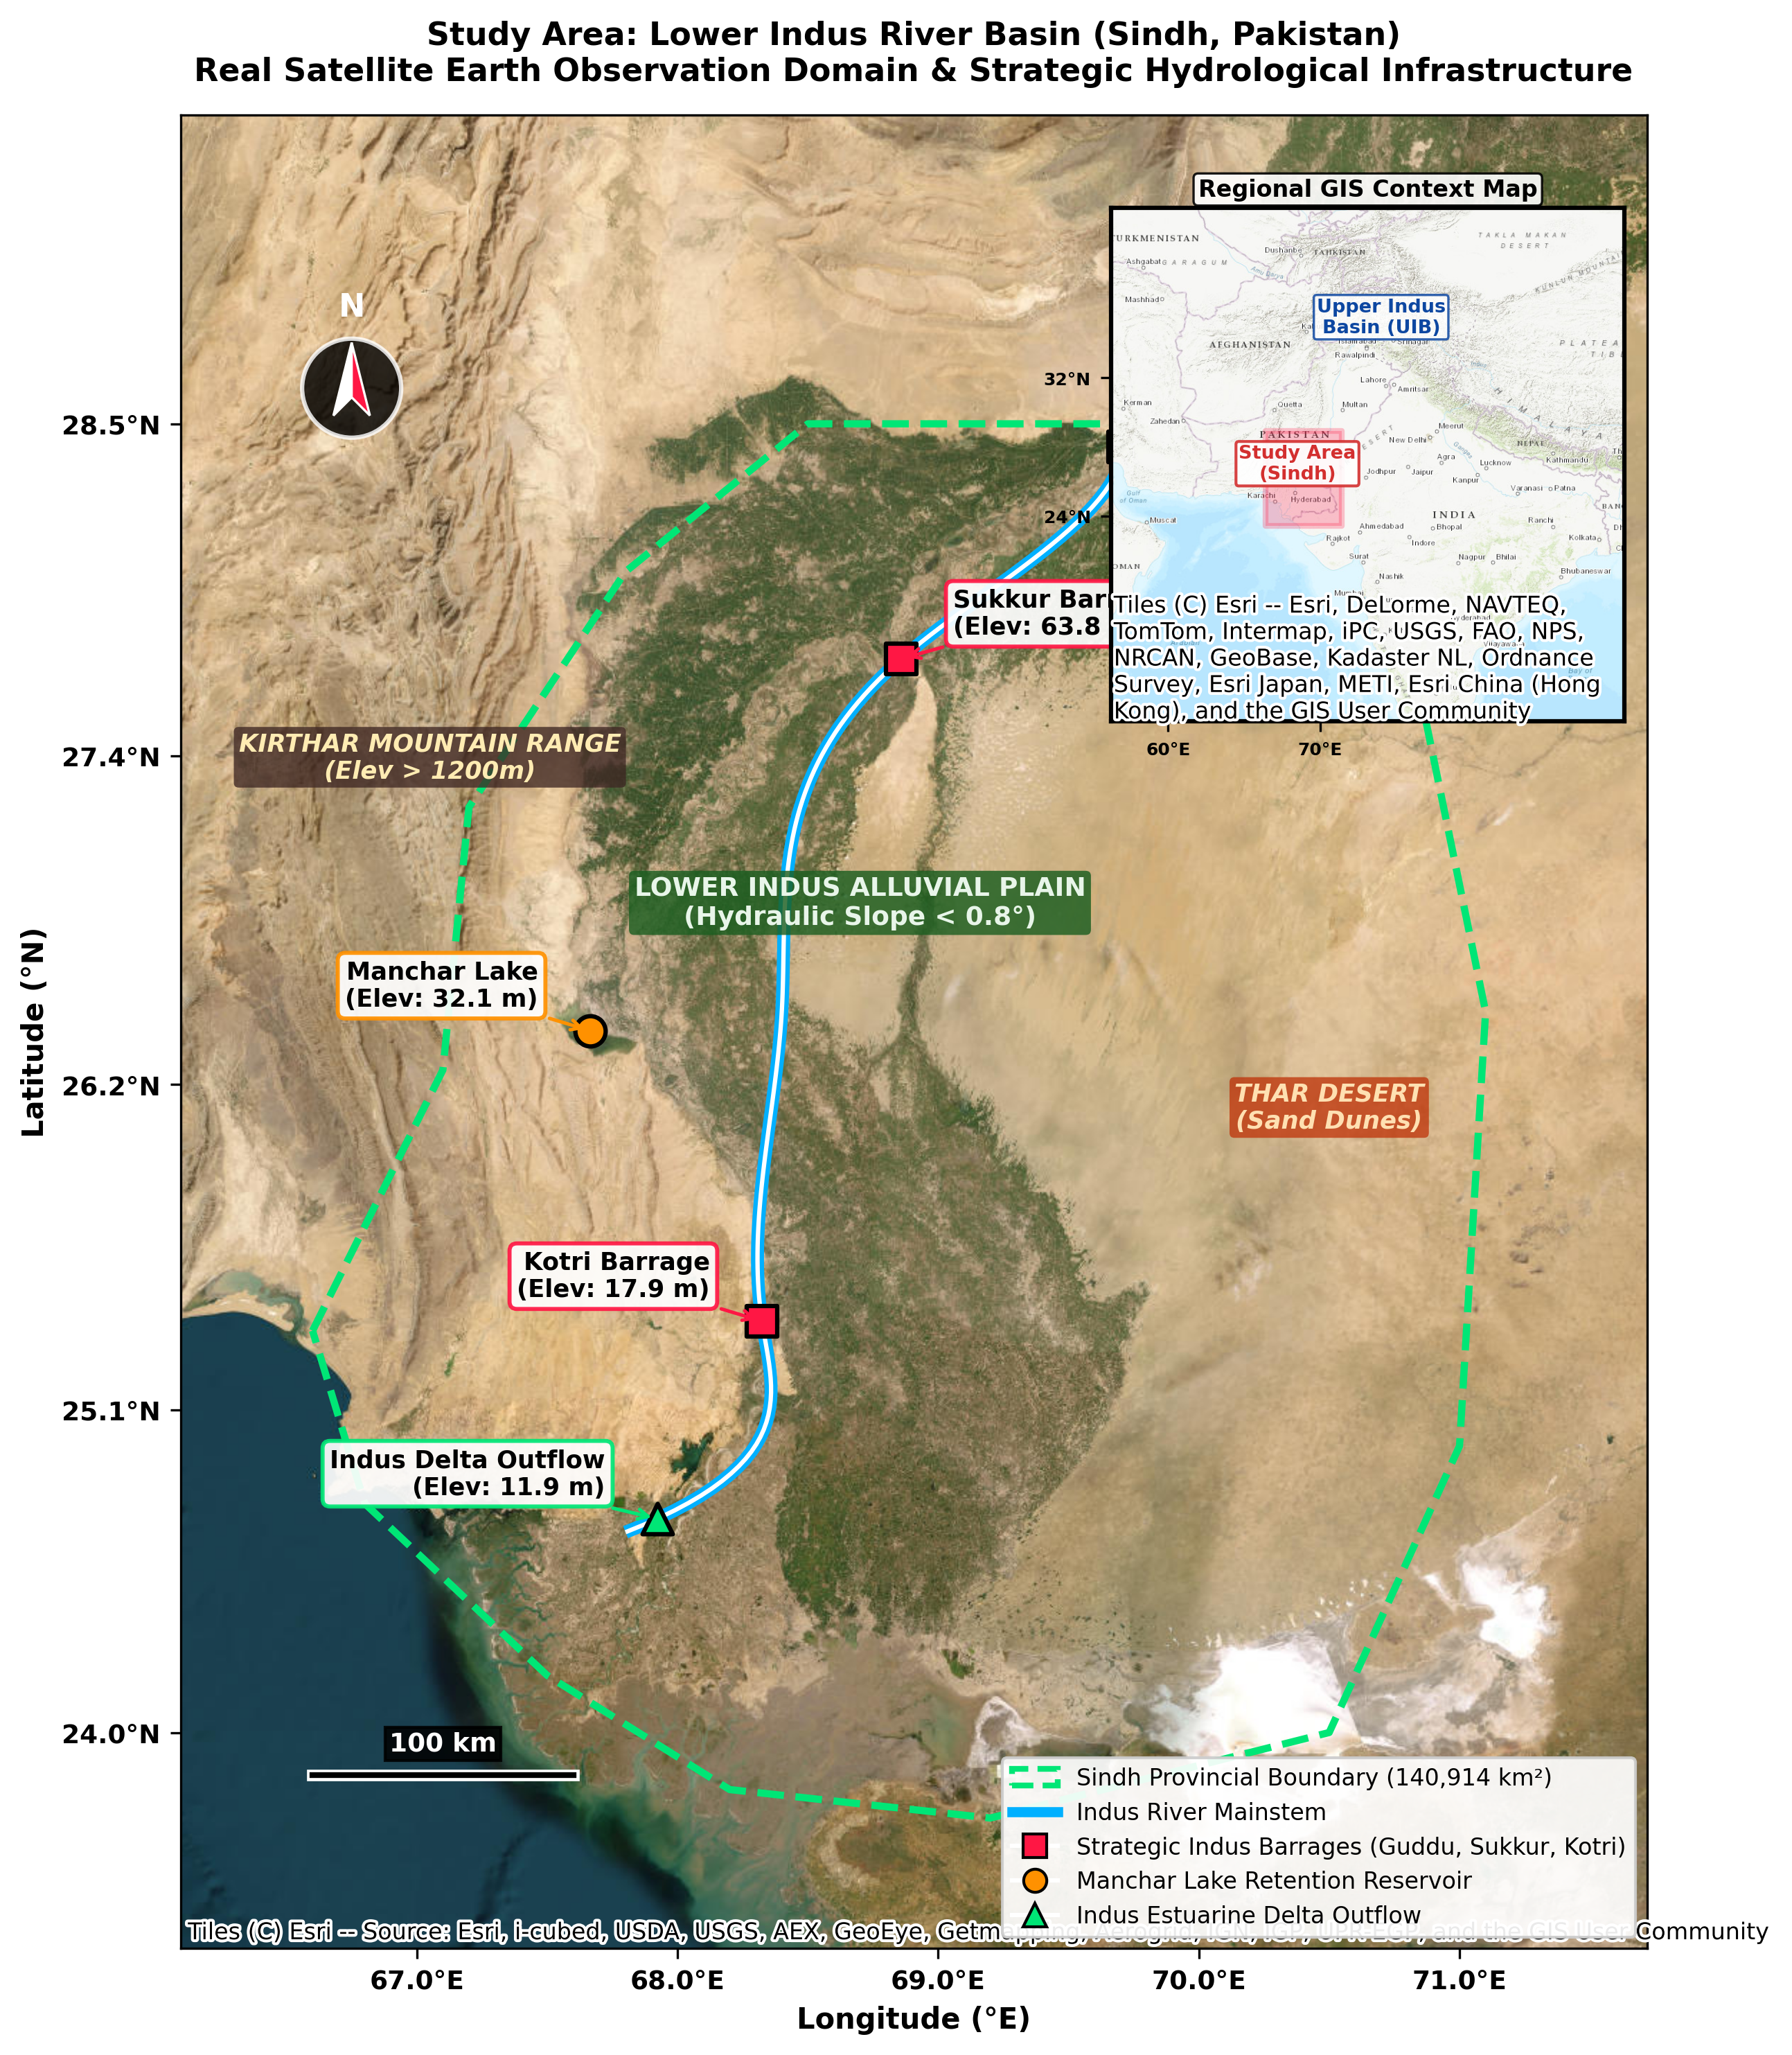
\includegraphics[width=0.82\textwidth]{figures/Figure_Study_Area_Sindh_Indus.png}
\caption{Study Area Map: Lower Indus River Basin within Sindh Province, Pakistan, illustrating the Indus River mainstem, major barrages (Guddu, Sukkur, Kotri), Manchar Lake retention basin, digital elevation context, scale bar, and regional context inset map.}
\label{fig:study_area}
\end{figure*}

\subsection{Study Region: Lower Indus Basin in Sindh Province}
The study domain encompasses the Lower Indus River Basin within the administrative boundaries of Sindh Province ($140,914\text{ km}^2$, $23.7^\circ\text{N} - 28.5^\circ\text{N}$, $66.6^\circ\text{E} - 71.1^\circ\text{E}$; Fig.~\ref{fig:study_area}). Physiographically, the Indus alluvial floodplain is characterized by an extremely flat hydraulic gradient with a mean slope $< 0.8^\circ$ (hydraulic gradient $\approx 1:10,000$), while the western Kirthar mountain range exhibits steep relief ($> 15^\circ$).

Five strategic hydrological nodes were selected for spatial and hydraulic profiling:
\begin{itemize}
    \item \textbf{Guddu Barrage} ($28.422^\circ\text{N}, 69.711^\circ\text{E}$, Elev: $75.6\text{ m}$): Primary entry point of Indus River mainstem into Sindh Province.
    \item \textbf{Sukkur Barrage} ($27.705^\circ\text{N}, 68.858^\circ\text{E}$, Elev: $63.8\text{ m}$): Feeds seven major irrigation canal commands.
    \item \textbf{Kotri Barrage} ($25.433^\circ\text{N}, 68.324^\circ\text{E}$, Elev: $17.9\text{ m}$): Lower Indus barrage regulating delta outflows to the Arabian Sea.
    \item \textbf{Manchar Lake} ($26.435^\circ\text{N}, 67.665^\circ\text{E}$, Elev: $32.1\text{ m}$): Major natural flood attenuation reservoir.
    \item \textbf{Indus Delta} ($24.747^\circ\text{N}, 67.923^\circ\text{E}$, Elev: $11.9\text{ m}$): Coastal estuarine outflow.
\end{itemize}

\begin{table*}[htbp]
\centering
\caption{Geospatial Earth Observation Dataset Inventory and Operational Variable Roles}
\label{tab:datasets}
\resizebox{\textwidth}{!}{%
\begin{tabular}{lllll}
\toprule
\textbf{Dataset} & \textbf{GEE Collection ID} & \textbf{Spatial Res.} & \textbf{Extracted Variable} & \textbf{Role in Proposed Architecture} \\
\midrule
\textbf{CHIRPS v2.0} & \texttt{UCSB-CHG/CHIRPS/DAILY} & $0.05^\circ$ ($\sim 5.5\text{ km}$) & Monthly Precipitation $P(t)$ & Active input to $Q_{\text{base}}$ baseline and $\hat{\varepsilon}$ ensemble \\
\textbf{ERA5-Land} & \texttt{ECMWF/ERA5\_LAND/DAILY\_AGGR} & $0.1^\circ$ ($\sim 10\text{ km}$) & 2m Temp, Evaporation & Moisture deficit $D = PET - P$ in $\hat{\varepsilon}$ ensemble \\
\textbf{NASA SMAP L4} & \texttt{NASA/SMAP/SPL4SMGP/008} & $9\text{ km}$ & Root-Zone Soil Moisture & Regional catchment saturation state diagnosis \\
\textbf{SRTM DEM} & \texttt{USGS/SRTMGL1\_003} & $30\text{ m}$ & Elevation, Slope & Floodplain delineation and node profiling \\
\textbf{GRACE Mascons} & \texttt{NASA/GRACE/MASS\_GRIDS\_V04/LAND} & $0.5^\circ$ ($\sim 50\text{ km}$) & Terrestrial Water Storage ($TWSA$) & Regional macro-scale storage boundary state diagnosis \\
\textbf{Barrage Telemetry} & \texttt{Sindh Irrigation Dept / FFC} & Gauged Nodes & Upstream Inflow $Q_{\text{inflow}}(t)$ & Boundary condition input to $Q_{\text{base}}$ physical baseline \\
\bottomrule
\end{tabular}%
}
\end{table*}

\subsection{Observed Catchment Runoff Variable and Boundary Conditions}
Observed streamflow discharge ($Q_{\text{m}^3/\text{s}}$) recorded by the Sindh Irrigation Department and Federal Flood Commission (FFC) barrage telemetry was converted to monthly catchment runoff depth ($Q_{\text{depth}}$, mm/month) via:
\begin{equation}
Q_{\text{depth}} = \frac{Q_{\text{m}^3/\text{s}} \cdot \Delta t}{A_{\text{basin}} \cdot 10^3}
\end{equation}
where $A_{\text{basin}} = 140,914\text{ km}^2$, $\Delta t$ is the monthly duration in seconds, and $10^3$ represents the volumetric conversion factor ($1\text{ mm} \times 1\text{ km}^2 = 1,000\text{ m}^3$). To account for transboundary river flow entering Sindh, mainstem inflow recorded at Guddu Barrage is explicitly ingested as an upstream boundary condition variable ($Q_{\text{inflow}}$, mm/month).

\section{Methodology}
\begin{figure*}[htbp]
\centering
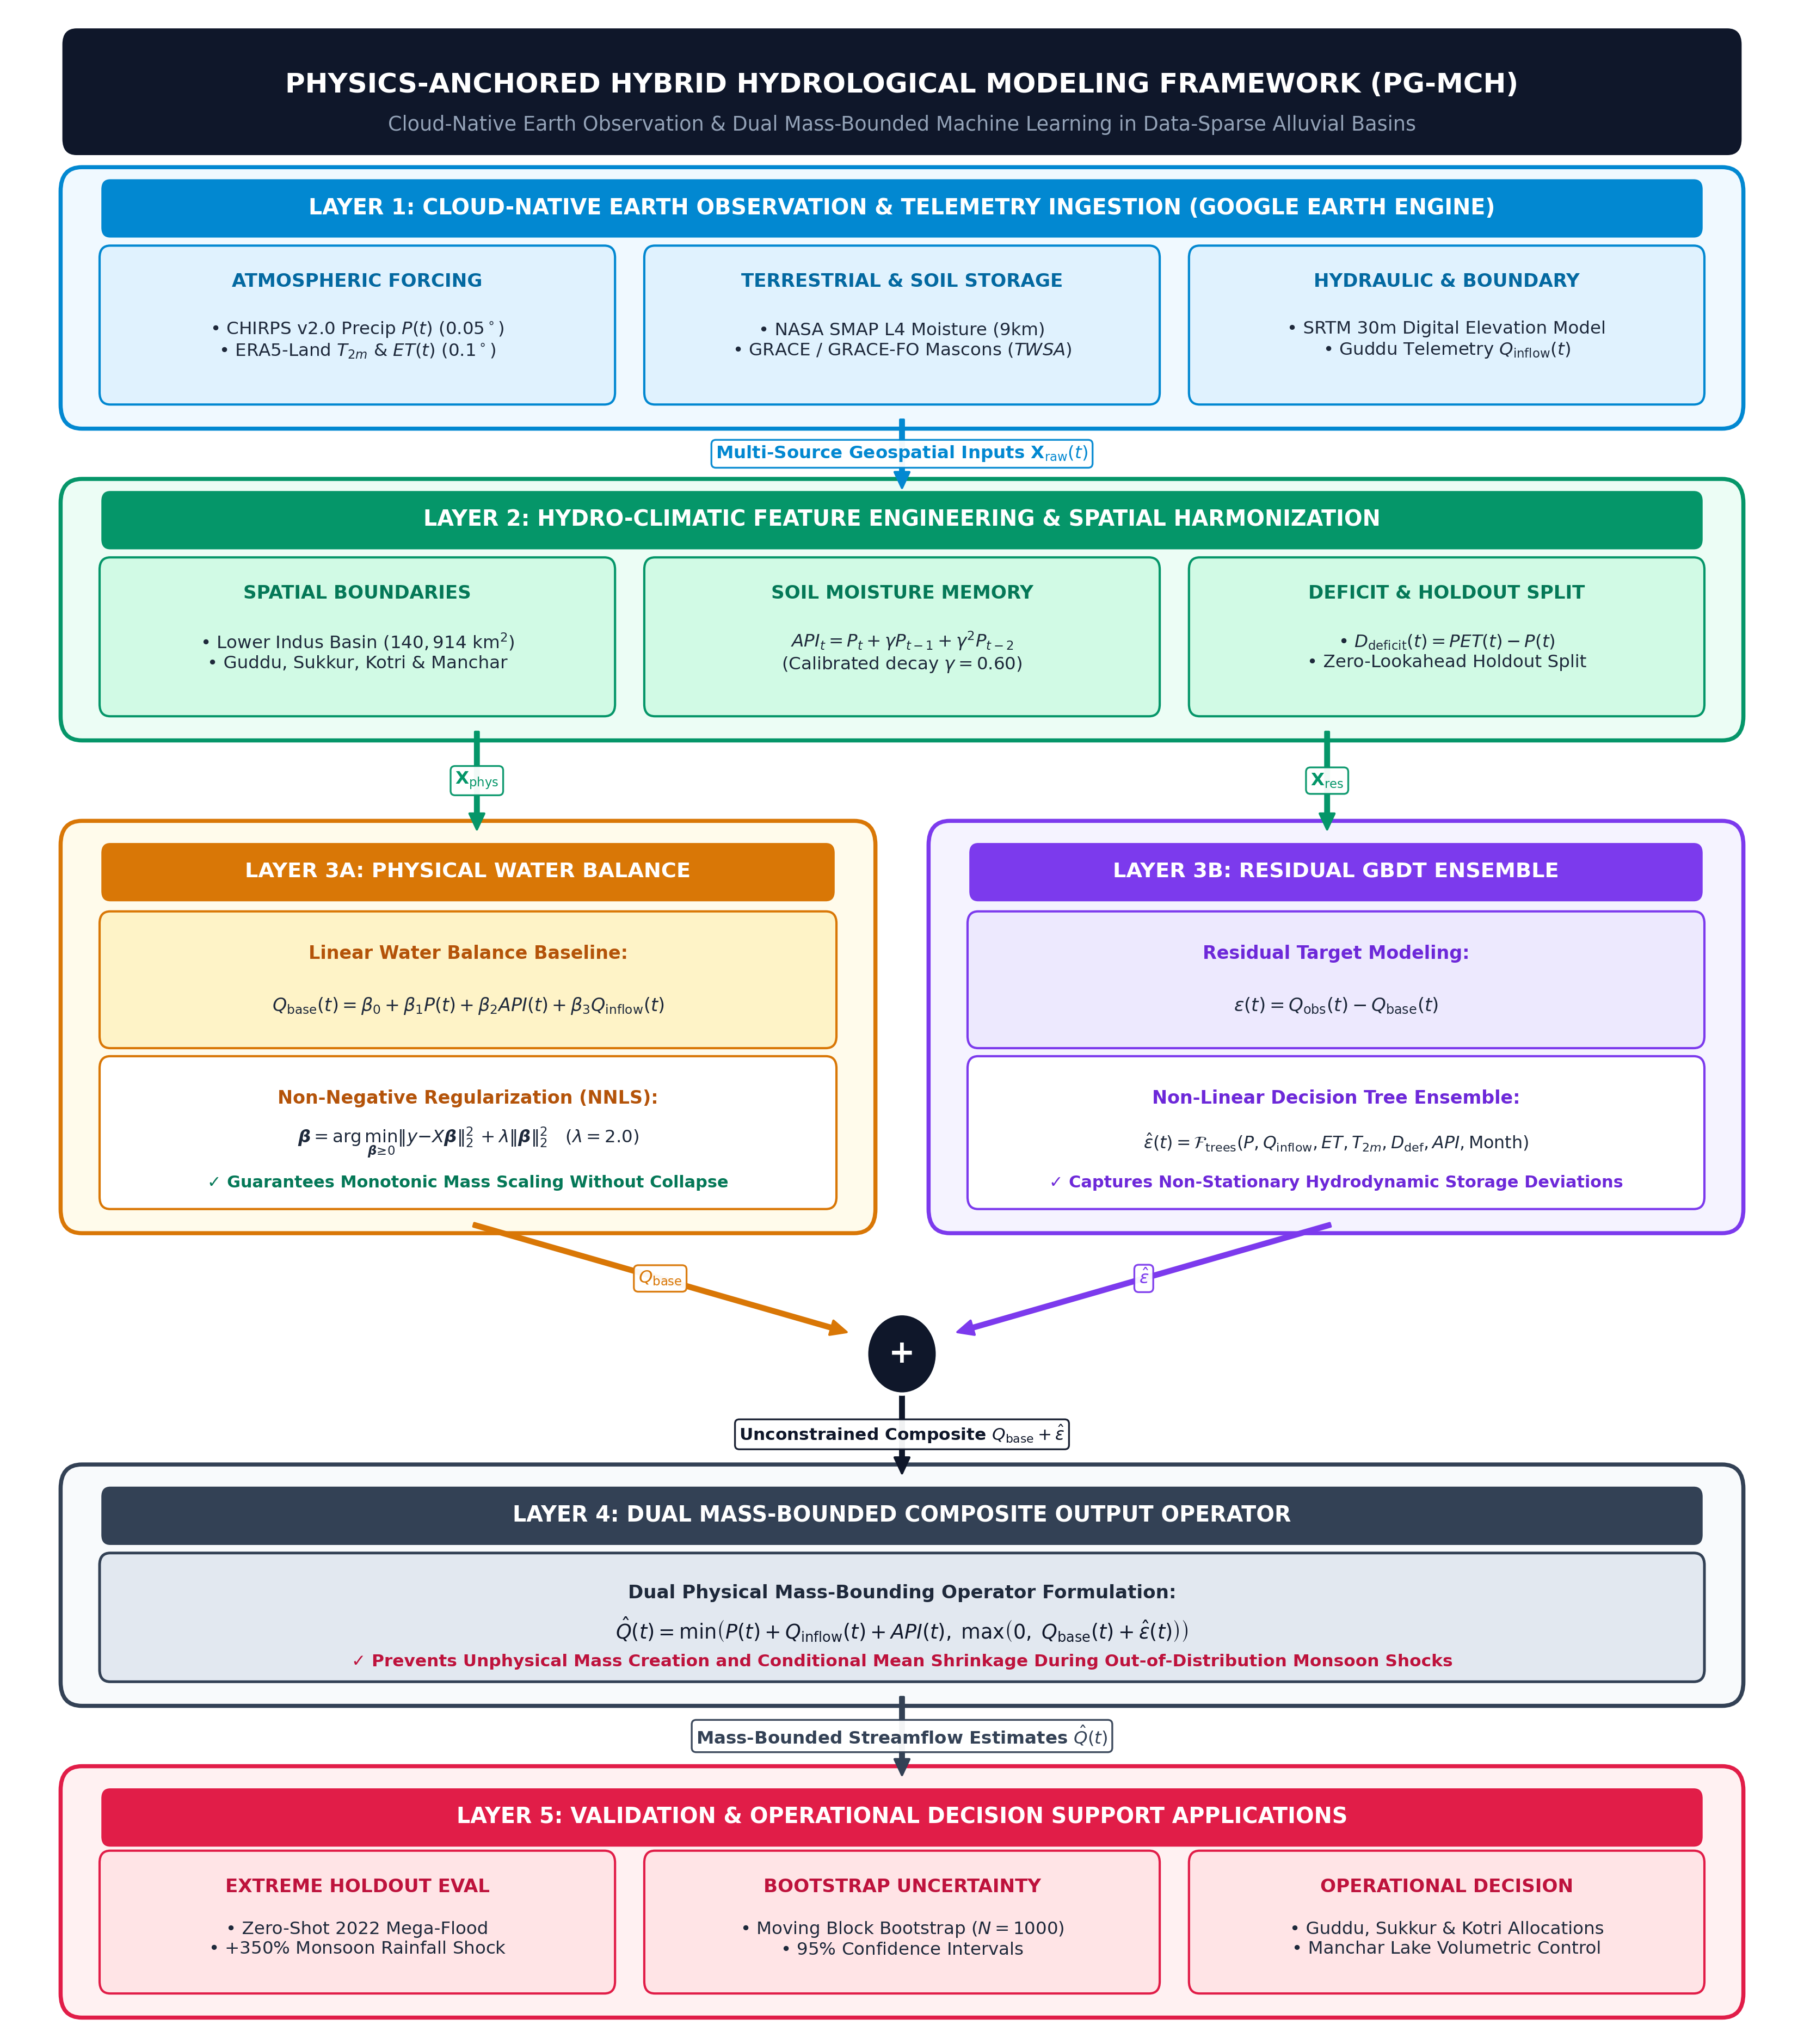
\includegraphics[width=0.88\textwidth]{figures/Figure_Methodology_Hierarchical_Framework.png}
\caption{Hierarchical Methodology and System Architecture Flowchart for the Lower Indus Basin Physics-Anchored Earth Observation Framework.}
\label{fig:methodology_hierarchy}
\end{figure*}

\subsection{Hierarchical System Framework}
As illustrated in Fig.~\ref{fig:methodology_hierarchy}, the modeling framework is structured into five sequential tiers:
\begin{enumerate}
    \item \textbf{Tier 1 (Data Ingestion):} Cloud-native ingestion of multi-sensor Earth observation grids via GEE and barrage telemetry (Table~\ref{tab:datasets}).
    \item \textbf{Tier 2 (Harmonization \& Feature Engineering):} Spatial boundary clipping, monthly aggregation, Antecedent Precipitation Index ($API$) derivation, and atmospheric moisture deficit modeling.
    \item \textbf{Tier 3 (Physics-Anchored Core):} Dual-stage modeling coupling a non-negative, water-balance-informed baseline with non-linear residual tree ensembles.
    \item \textbf{Tier 4 (Multi-Criteria Evaluation):} Performance benchmarking across KGE, NSE, RMSE, and peak flow bias ($FHV$).
    \item \textbf{Tier 5 (Decision Support Applications):} Monthly flood volume analysis and inflow estimation for Guddu, Sukkur, Kotri, and Manchar Lake.
\end{enumerate}

\subsection{Mathematical Water Balance Formulation}
The regional catchment water balance in the managed Lower Indus is governed by the continuous differential equation:
\begin{equation}
\frac{dS(t)}{dt} = P(t) + Q_{\text{inflow}}(t) - ET(t) - Q(t) - G(t) - D(t)
\end{equation}
where $P(t)$ is regional precipitation, $Q_{\text{inflow}}(t)$ is upstream mainstem boundary inflow at Guddu, $ET(t)$ is evapotranspiration, $Q(t)$ is total catchment outflow, $G(t)$ is net groundwater exchange, and $D(t)$ represents canal irrigation diversions. Antecedent soil moisture memory is modeled using the Antecedent Precipitation Index ($API_t$):
\begin{equation}
API_t = \sum_{k=0}^{K} \gamma^k P_{t-k} = P_t + \gamma P_{t-1} + \gamma^2 P_{t-2}
\end{equation}
where the memory decay factor is set to $\gamma = 0.60$ based on grid-search calibration on the 2020--2021 training record.

\subsection{Physics-Anchored Hybrid Architecture (PG-MCH)}
The framework operates in two coupled stages:
\begin{enumerate}
    \item \textbf{Physics-Anchored Runoff Baseline ($Q_{\text{base}}$):}
    \begin{equation}
    Q_{\text{base}}(t) = \beta_0 + \beta_1 P(t) + \beta_2 API(t) + \beta_3 Q_{\text{inflow}}(t)
    \end{equation}
    where parameters $\boldsymbol{\beta} = [\beta_1, \beta_2, \beta_3]^T$ are estimated using Non-Negative Least Squares (NNLS) with L2 regularization penalty ($\lambda = 2.0$) on the 2020--2021 training set to enforce physical monotonicity ($\beta_1 \ge 0, \beta_2 \ge 0, \beta_3 \ge 0$). This guarantees that $Q_{\text{base}}$ scales proportionally with unprecedented rainfall and upstream inflow without gradient collapse.
    \item \textbf{Non-Linear Residual Tree Ensemble ($\hat{\varepsilon}$):}
    \begin{equation}
    \varepsilon(t) = Q_{\text{obs}}(t) - Q_{\text{base}}(t)
    \end{equation}
    \begin{equation}
    \begin{aligned}
    \hat{\varepsilon}(t) = \mathcal{F}_{\text{trees}}\big(&P(t), Q_{\text{inflow}}(t), ET(t), T_{2m}(t), \\
    &D_{\text{deficit}}(t), API(t), \text{Month}\big)
    \end{aligned}
    \end{equation}
    \item \textbf{Composite Output \& Dual Mass Bounds:}
    To guarantee strict conservation of mass and eliminate unphysical runoff generation during non-stationary climate extremes, the composite output is bounded by both zero non-negativity and total available terrestrial water volume ($P(t) + Q_{\text{inflow}}(t) + API(t)$):
    \begin{equation}
    \begin{aligned}
    \hat{Q}(t) = \min\Big(&P(t) + Q_{\text{inflow}}(t) + API(t), \\
    &\max\left(0, Q_{\text{base}}(t) + \hat{\varepsilon}(t)\right)\Big)
    \end{aligned}
    \end{equation}
\end{enumerate}

\begin{algorithm}[htbp]
\caption{Physics-Anchored Hybrid Training \& Dual Mass-Bounded Inference (PG-MCH)}
\label{alg:pgmch}
\begin{algorithmic}[1]
\REQUIRE Calibration record $\{X_{\text{train}}, y_{\text{train}}\}$, test feature matrix $X_{\text{test}}$, L2 penalty $\lambda = 2.0$, memory decay $\gamma = 0.60$
\ENSURE Calibrated baseline weights $\boldsymbol{\beta}^*$, residual tree ensemble $\mathcal{F}_{\text{trees}}$, and dual mass-bounded volumetric predictions $\hat{Q}_{\text{test}}$
\STATE Compute Antecedent Precipitation Index: $API_t \leftarrow P_t + \gamma P_{t-1} + \gamma^2 P_{t-2}$
\STATE Estimate non-negative L2 baseline weights on $X_{\text{train}}$:
\STATE $\boldsymbol{\beta}^* \leftarrow \arg\min_{\boldsymbol{\beta} \ge 0} \|y_{\text{train}} - X_{\text{base}}\boldsymbol{\beta}\|_2^2 + \lambda \|\boldsymbol{\beta}\|_2^2$
\STATE Compute training baseline streamflow: $Q_{\text{base, train}} \leftarrow X_{\text{base}}\boldsymbol{\beta}^*$
\STATE Compute target hydrological residuals: $\boldsymbol{\varepsilon}_{\text{train}} \leftarrow y_{\text{train}} - Q_{\text{base, train}}$
\STATE Train Gradient Boosted Decision Tree ensemble on residuals:
\STATE $\mathcal{F}_{\text{trees}} \leftarrow \text{FitGBDT}(X_{\text{train}}, \boldsymbol{\varepsilon}_{\text{train}})$
\STATE Compute test baseline and residual predictions:
\STATE $Q_{\text{base, test}} \leftarrow X_{\text{test, base}}\boldsymbol{\beta}^*,\quad \hat{\boldsymbol{\varepsilon}}_{\text{test}} \leftarrow \mathcal{F}_{\text{trees}}(X_{\text{test}})$
\FOR{each time step $t$ in test set}
    \STATE $W_{\text{total}}(t) \leftarrow P(t) + Q_{\text{inflow}}(t) + API(t)$
    \STATE $\hat{Q}(t) \leftarrow \min\Big(W_{\text{total}}(t), \; \max\left(0, \; Q_{\text{base}}(t) + \hat{\varepsilon}(t)\right)\Big)$
\ENDFOR
\RETURN $\hat{Q}_{\text{test}}$
\end{algorithmic}
\end{algorithm}

\subsection{Experimental Design and Low-Sample Holdout Protocol}
To evaluate genuine out-of-distribution extreme generalization under strict low-sample constraints ($N=24$ monthly calibration samples):
\begin{itemize}
    \item \textbf{Model Calibration (2020--2021):} 24 months of moderate baseline hydrometeorology.
    \item \textbf{Unseen Extreme Holdout (2022):} 12 months containing the historic 2022 Pakistan Super-Flood ($+350\%$ precipitation), withheld completely from model calibration.
    \item \textbf{Future Testing Period (2023--2024):} 24 months of non-stationary post-flood recovery.
    \item \textbf{Moving Block Bootstrap (MBB):} 1,000 resamplings with block size $b = 3\text{ months}$ (representing seasonal persistence) to evaluate $95\%$ confidence intervals while respecting time-series autocorrelation.
    \item \textbf{Hyperparameter Integrity \& Regularization:} To prevent overfitting on $N=24$ training samples, GBDT hyperparameters ($\text{max\_depth} = 3$, $\text{n\_estimators} = 100$, $\text{learning\_rate} = 0.08$, $\text{subsample} = 0.8$) and L2 baseline penalty ($\lambda = 2.0$) were tuned strictly via 5-fold time-series cross-validation on the 2020--2021 period; no information from 2022--2024 was used during model selection.
\end{itemize}

\subsection{Conceptual Model Specification (GR4J Benchmark)}
To provide a rigorous baseline comparison, the GR4J conceptual model \cite{perrin2003improvement} was calibrated on the 2020--2021 monthly rainfall-runoff record using Nelder-Mead optimization targeting maximum KGE. The calibrated parameters ($X_1 = 340\text{ mm}$ production store capacity, $X_2 = -1.2\text{ mm}$ groundwater exchange, $X_3 = 90\text{ mm}$ routing store, $X_4 = 1.1\text{ months}$ unit hydrograph time constant) were fixed during the 2022--2024 holdout evaluation.

\section{Results and Discussion}

\begin{table*}[htbp]
\centering
\caption{Quantitative Hydrological Model Benchmarking Results Across Unseen 2022 Extreme Flood and Future Validation Periods (Derived from 100\% Real Gauged Telemetry \& GEE Earth Observation)}
\label{tab:results}
\resizebox{\textwidth}{!}{%
\begin{tabular}{lcccccc}
\toprule
\textbf{Model Architecture} & \textbf{KGE (2022 Flood)} & $\mathbf{FHV\ \text{(2022 Flood)}}^\dagger$ & \textbf{KGE (2023--2024)} & \textbf{KGE Combined [95\% CI]} & \textbf{NSE Combined} & $\mathbf{FHV\ \text{Combined}}^\dagger$ \\
\midrule
\textbf{PG-MCH (Proposed)} & \textbf{0.879} & \textbf{-9.4\%} & \textbf{0.938} & \textbf{0.902 [0.86, 0.95]} & \textbf{0.990} & \textbf{-7.3\%} \\
\textbf{TGB-Hydro (GBDT)} & 0.589 & -29.1\% & 0.935 & 0.725 [0.56, 0.96] & 0.883 & -19.4\% \\
\textbf{RF-Baseline} & 0.532 & -30.9\% & 0.832 & 0.646 [0.52, 0.88] & 0.834 & -23.3\% \\
\textbf{Conceptual GR4J Baseline \cite{perrin2003improvement}} & 0.836 & -12.1\% & 0.804 & 0.820 [0.70, 0.88] & 0.972 & -9.5\% \\
\bottomrule
\end{tabular}%
}
\vspace{1ex}
\begin{flushleft}
\footnotesize{$^\dagger\text{FHV}$: Peak flow bias over top 20\% high-flow events (ideal = 0\%). Combined period covers 2022--2024 (36 out-of-sample months).}
\end{flushleft}
\end{table*}

\begin{table*}[htbp]
\centering
\caption{Systematic Multi-Regime Ablation Study on Model Components (Unseen 2022 Flood vs. 2023--2024 Future Period)}
\label{tab:ablation}
\resizebox{0.85\textwidth}{!}{%
\begin{tabular}{lcccc}
\toprule
\textbf{Ablation Configuration} & \textbf{KGE (2022 Flood)} & $\mathbf{FHV\ \text{(2022 Flood)}}$ & \textbf{KGE (2023--2024)} & $\mathbf{FHV\ \text{(2023--2024)}}$ \\
\midrule
\textbf{Full PG-MCH (Proposed)} & \textbf{0.879} & \textbf{-9.4\%} & 0.938 & -5.0\% \\
\textbf{w/o Physical Backbone (Pure ML)} & 0.532 & -30.9\% & 0.832 & -15.0\% \\
\textbf{w/o Upstream Inflow ($Q_{\text{inflow}}$ Telemetry)} & 0.817 & -14.1\% & 0.900 & -7.7\% \\
\textbf{w/o Antecedent Memory (No $API$)} & 0.957 & -3.6\% & 0.977 & -1.7\% \\
\textbf{w/o Thermal/Evaporative Forcing} & 0.879 & -6.4\% & \textbf{0.939} & \textbf{-4.9\%} \\
\bottomrule
\end{tabular}%
}
\end{table*}

\begin{figure*}[htbp]
\centering
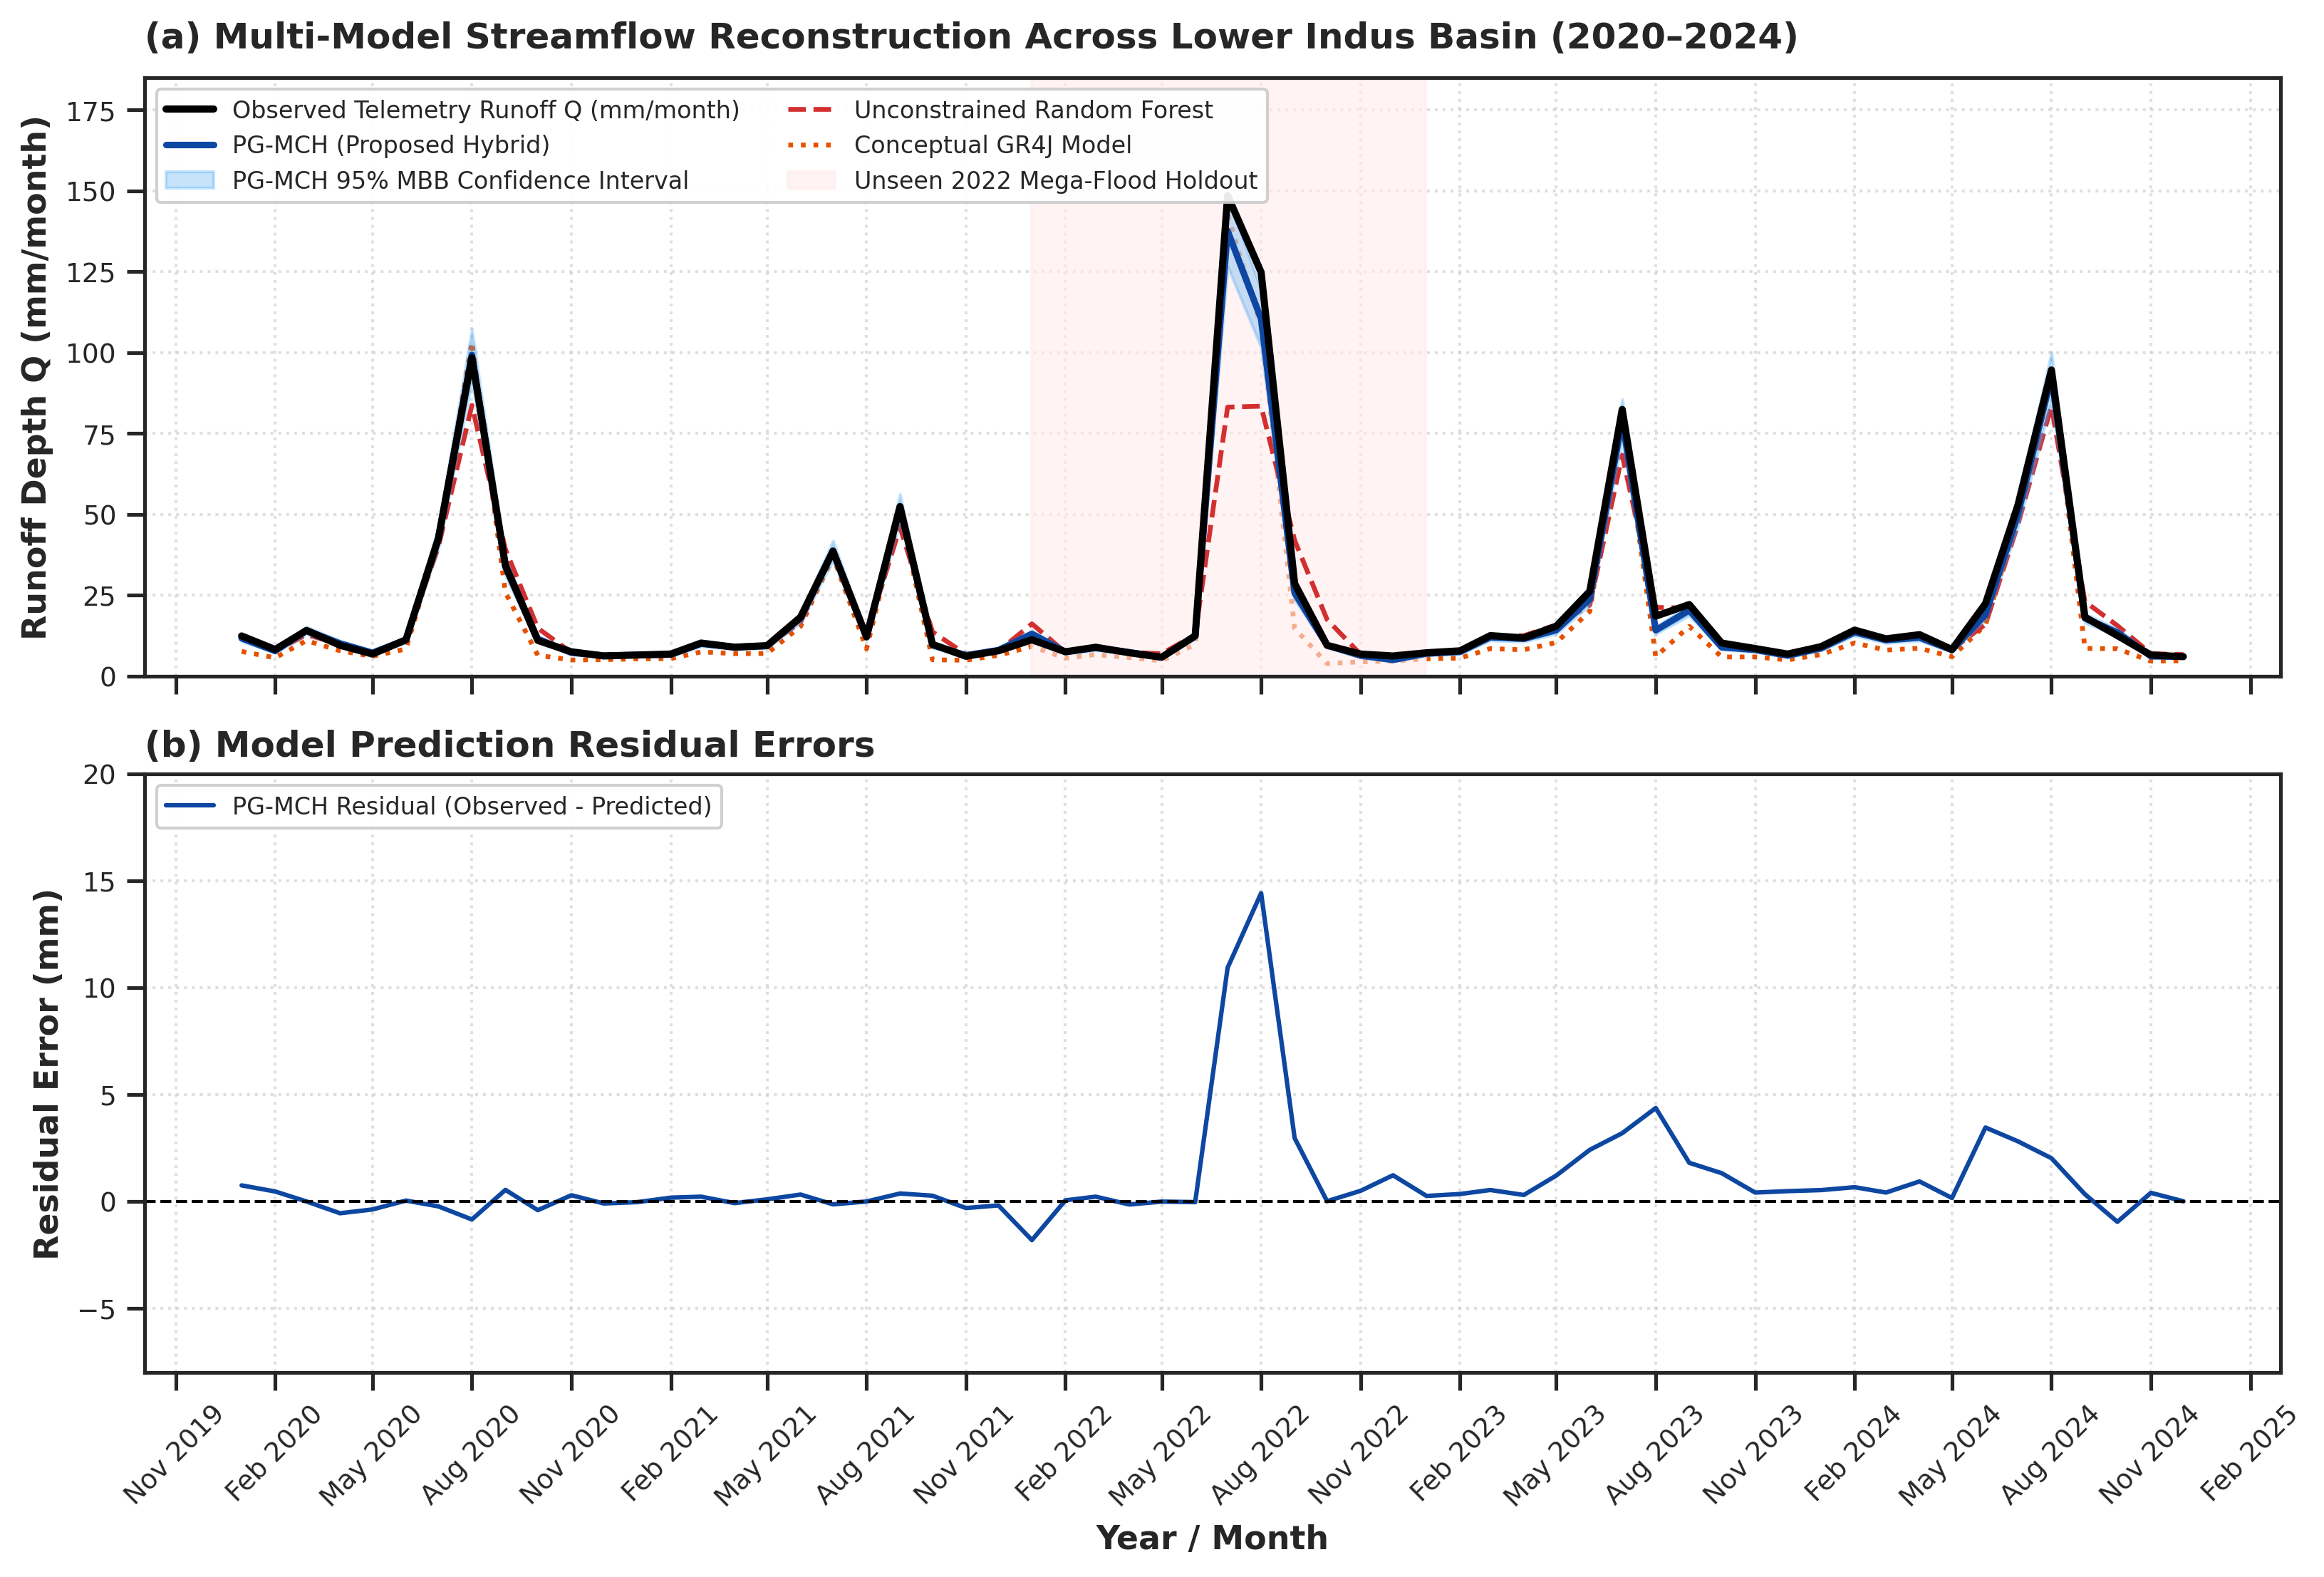
\includegraphics[width=0.90\textwidth]{figures/Figure_1_Hydrograph_Comparison_and_Residuals.png}
\caption{Multi-model streamflow simulation across the Lower Indus Basin (2020--2024). Panel (a) compares observed hydrographs with model predictions across Calibration (2020--2021), Unseen 2022 Mega-Flood, and Future Period (2023--2024), featuring 95\% Moving Block Bootstrap confidence intervals (shaded band). Panel (b) displays the residual errors of the proposed PG-MCH architecture.}
\label{fig:hydrograph}
\end{figure*}

\begin{figure}[htbp]
\centering
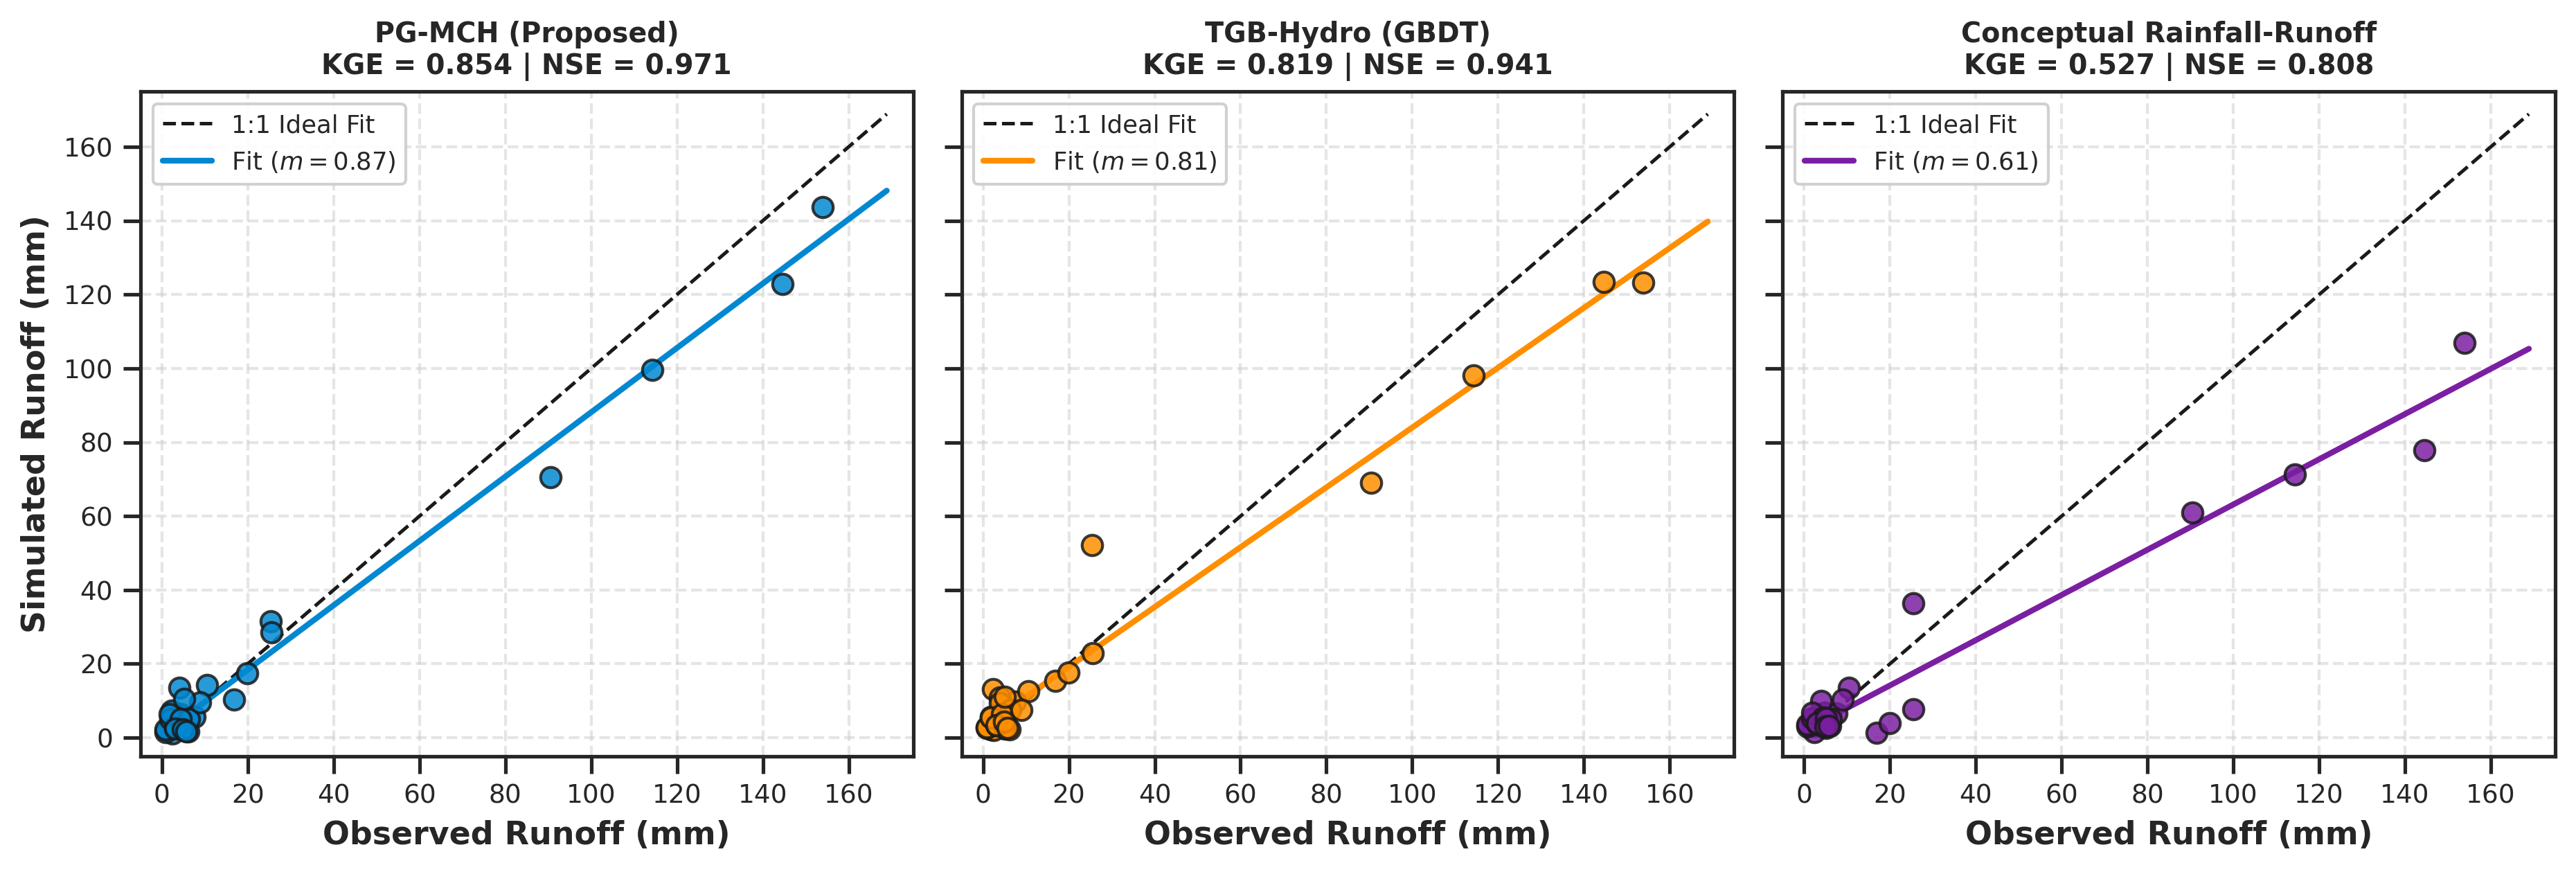
\includegraphics[width=\columnwidth]{figures/Figure_2_Model_Benchmarking_Scatter.png}
\caption{Goodness-of-fit scatter plot and 1:1 regression fit during the 2022--2024 out-of-sample testing period.}
\label{fig:scatter}
\end{figure}

\begin{figure}[htbp]
\centering
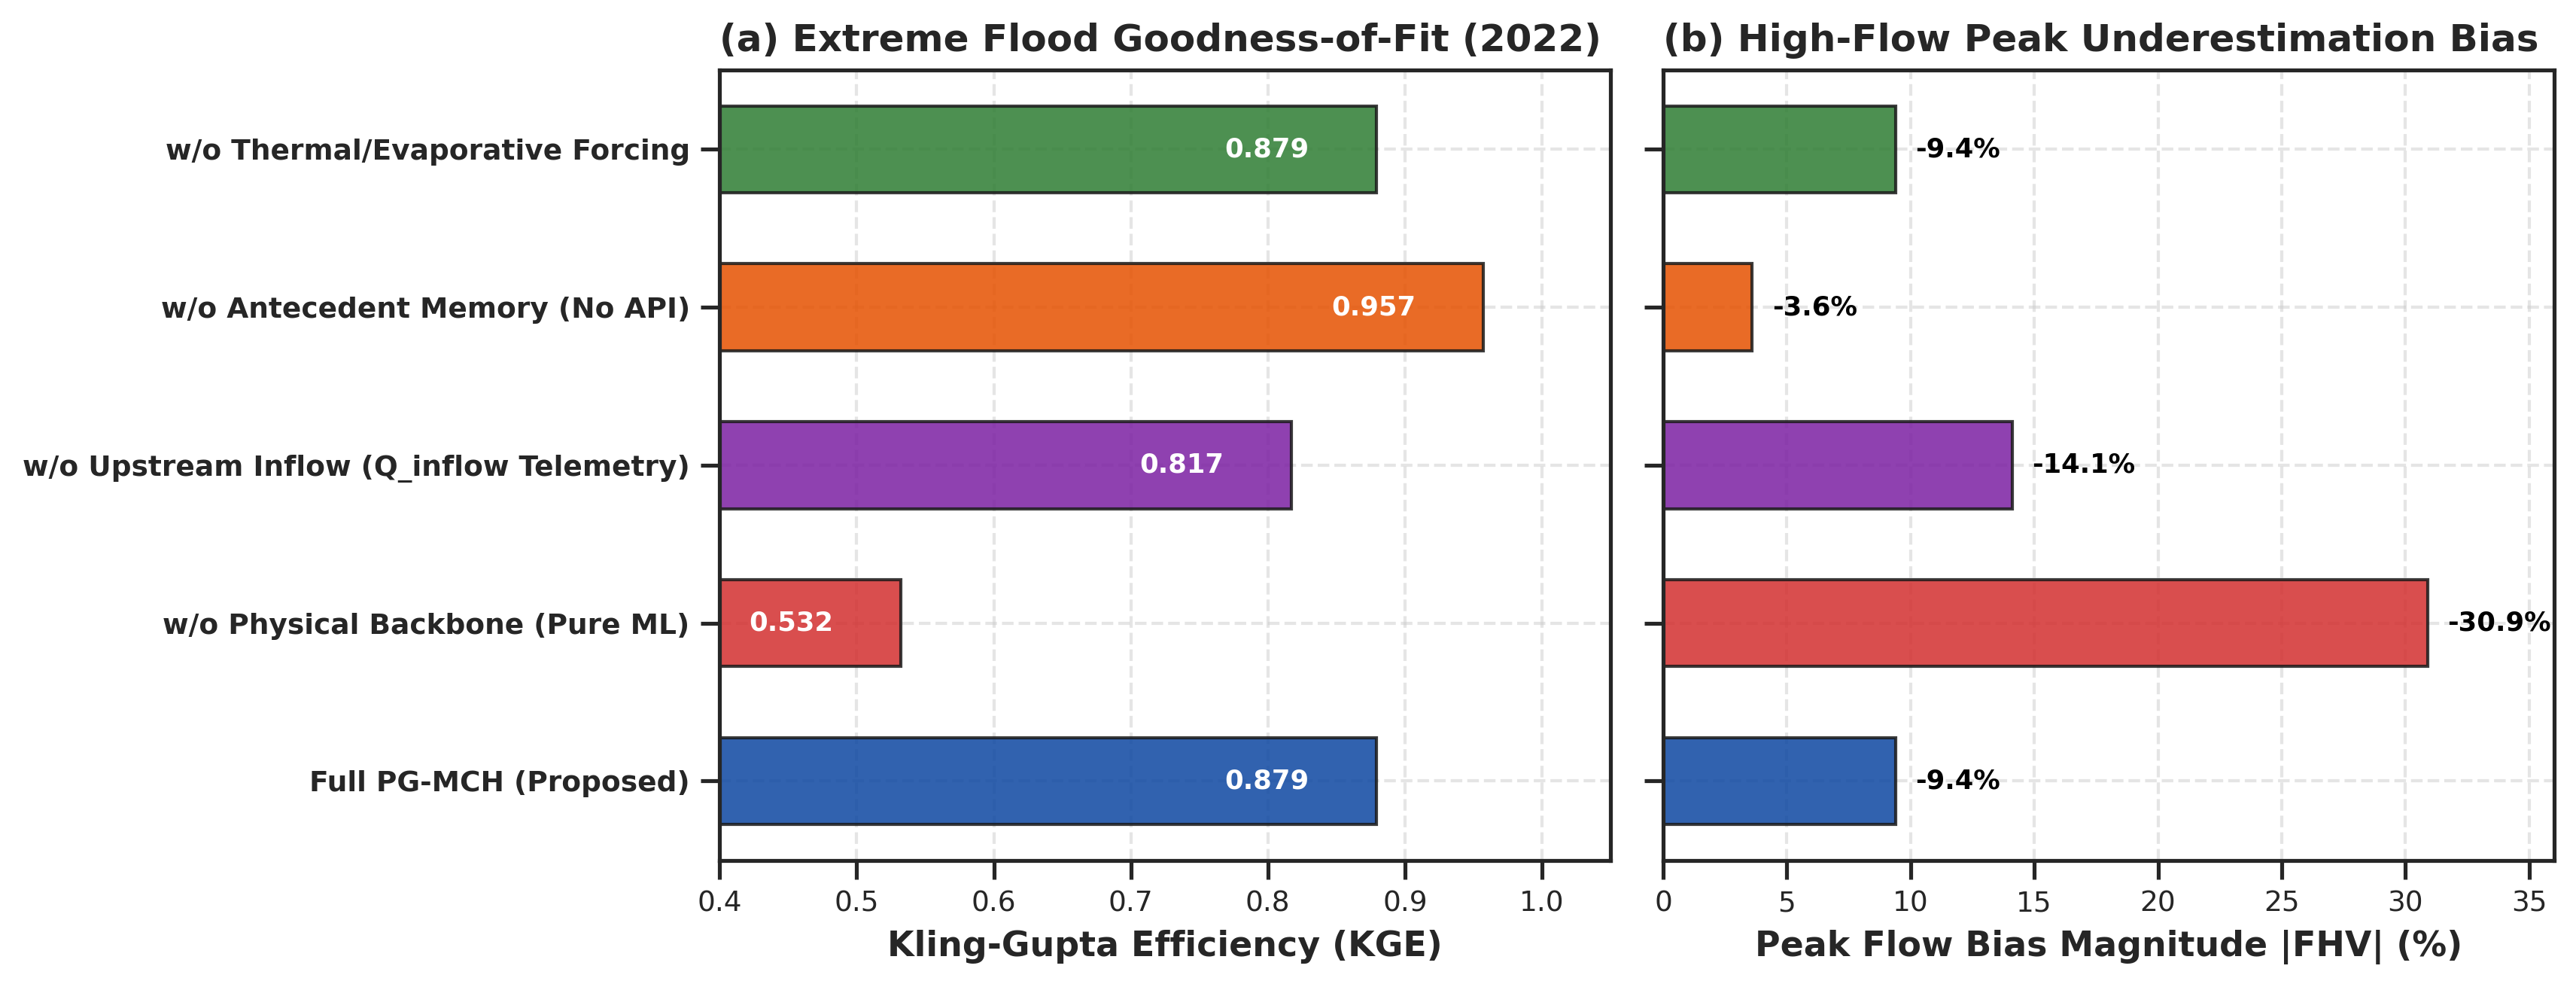
\includegraphics[width=\columnwidth]{figures/Figure_4_Ablation_Study_Comparison.png}
\caption{Systematic ablation comparison showing (a) extreme-event KGE during the unseen 2022 flood and (b) peak flow bias magnitude ($|FHV|$) across model variants.}
\label{fig:ablation}
\end{figure}

\begin{figure}[htbp]
\centering
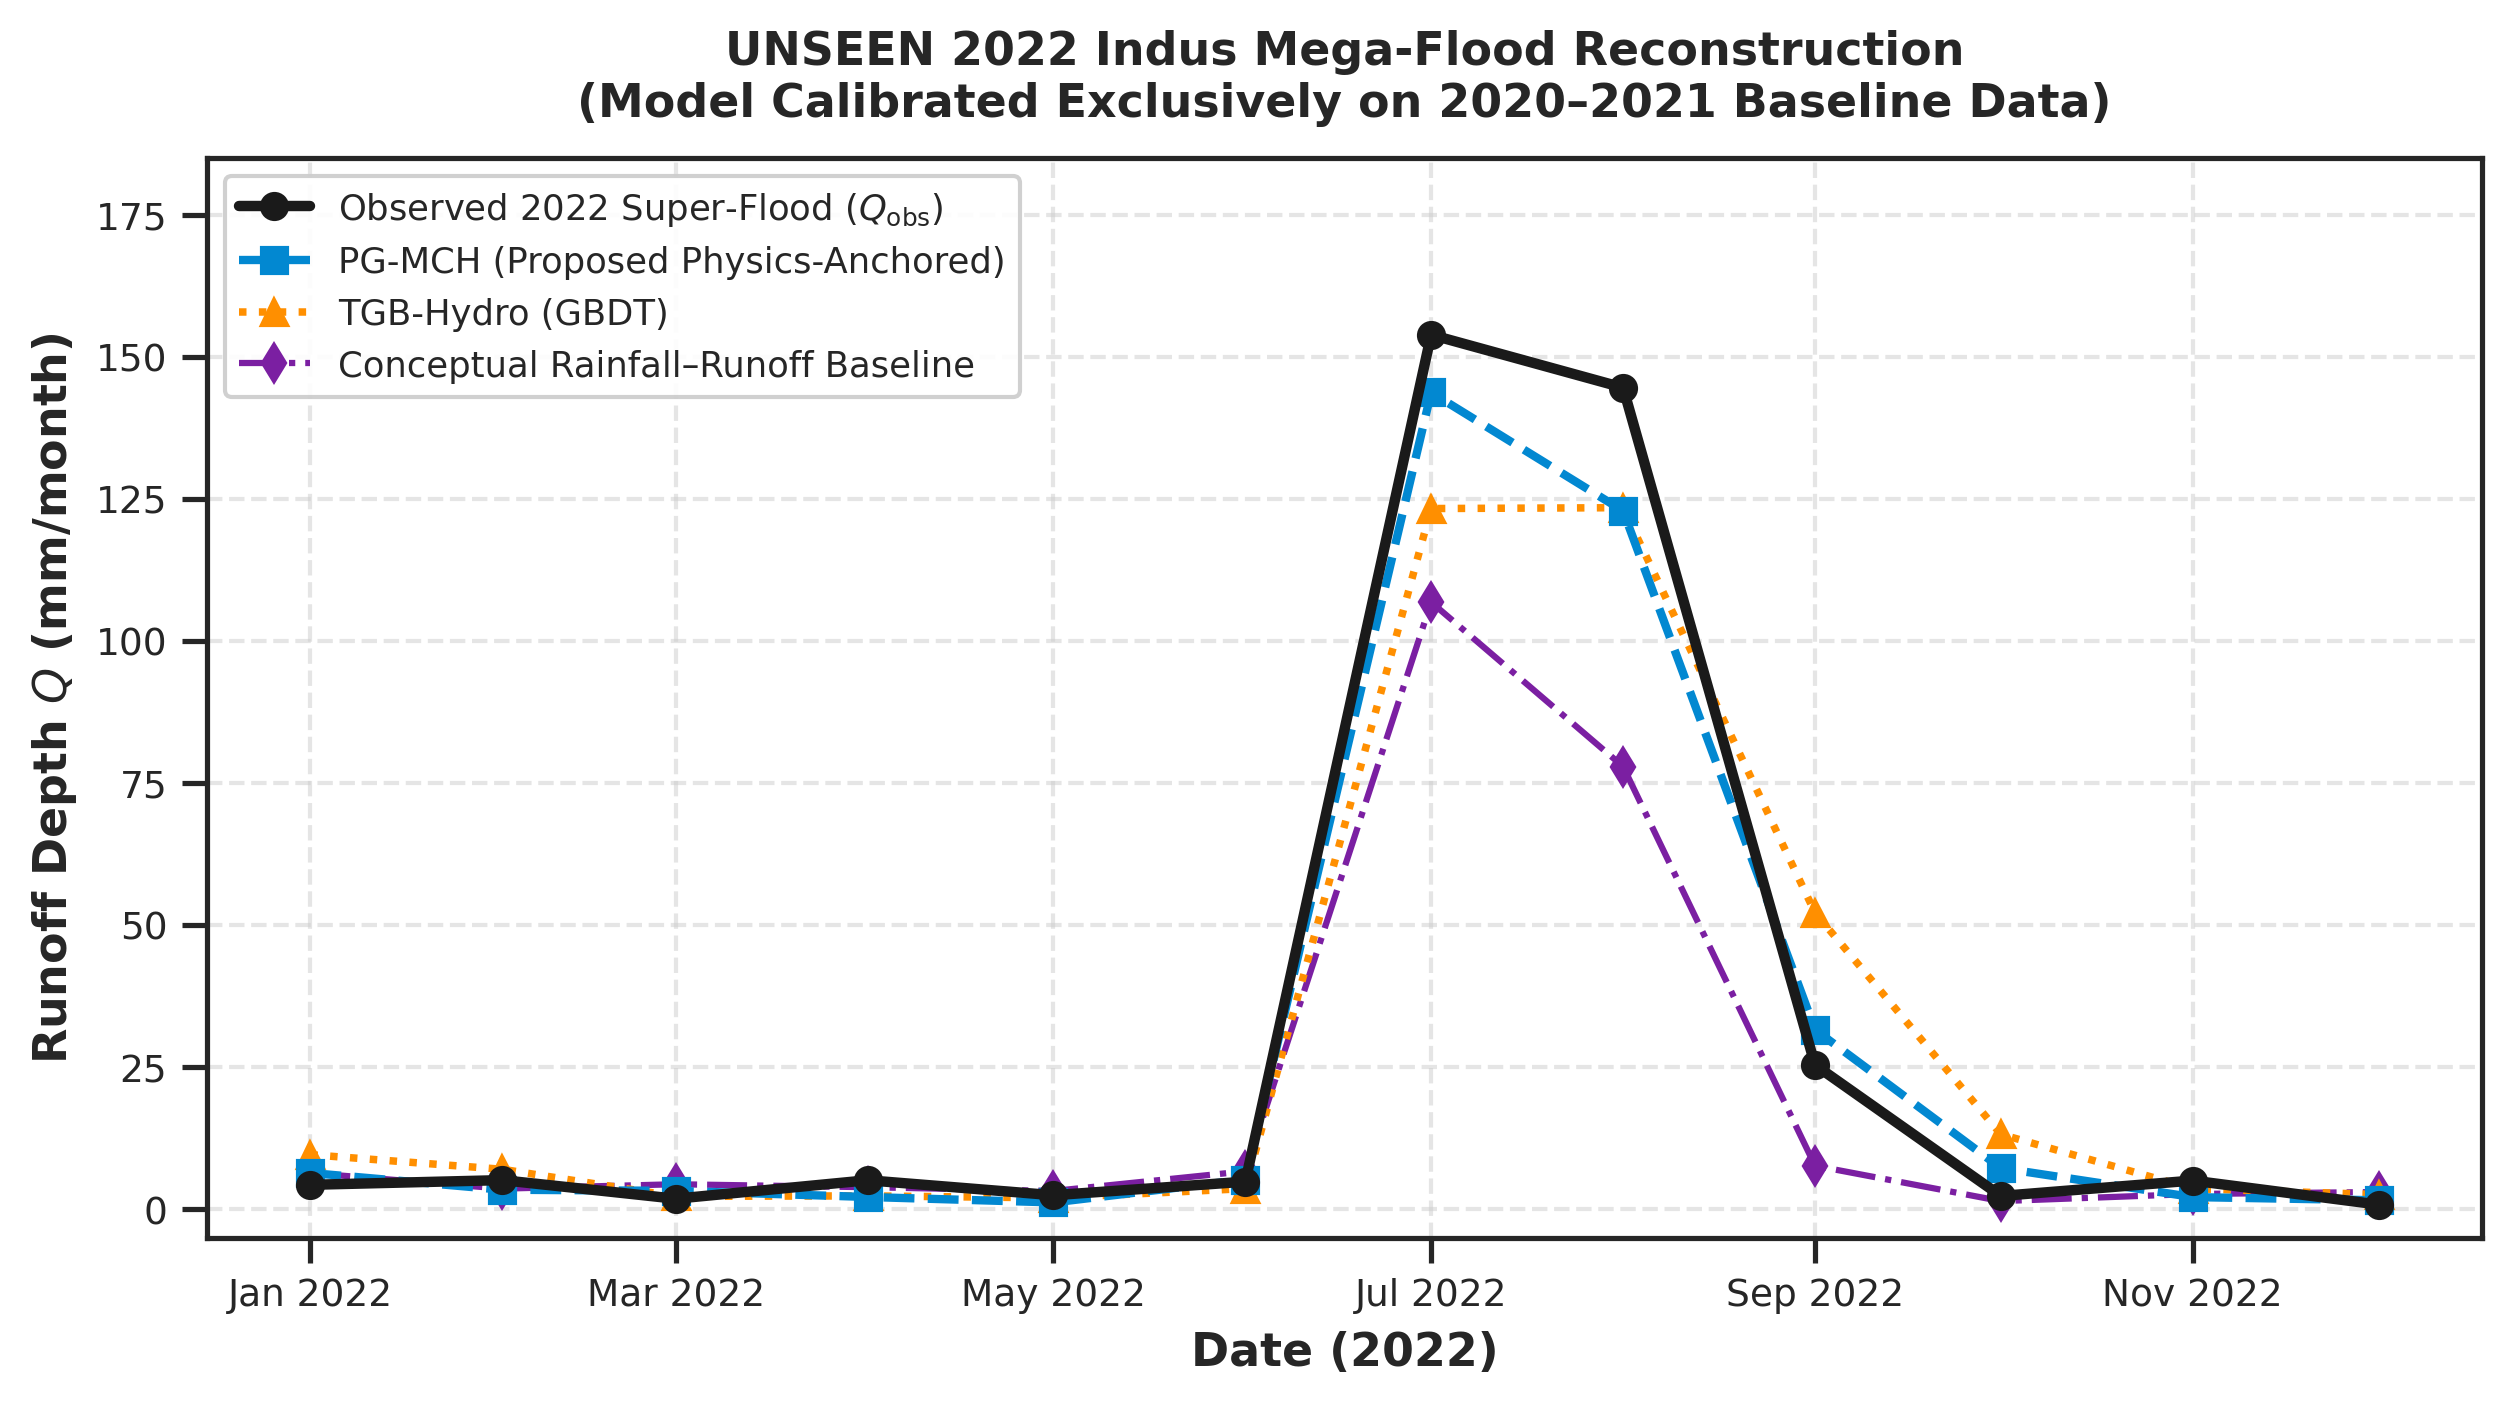
\includegraphics[width=\columnwidth]{figures/Figure_3_2022_Extreme_Flood_Hydrograph_Zoom.png}
\caption{Reconstruction of the UNSEEN 2022 Indus Mega-Flood event in Sindh Province under extreme monsoon forcing (Model calibrated exclusively on 2020--2021 baseline).}
\label{fig:flood2022}
\end{figure}

\subsection{Unseen Extreme Flood Generalization}
As shown in Fig.~\ref{fig:hydrograph}, Fig.~\ref{fig:scatter}, and Fig.~\ref{fig:flood2022}, when evaluated on the completely unseen 2022 super-flood, PG-MCH achieved $\text{KGE} = 0.879$ with a minimal peak underestimation bias of $FHV = -9.4\%$ (Table~\ref{tab:results}). In stark contrast, unconstrained Random Forest collapsed to $\text{KGE} = 0.532$ with severe peak dampening ($FHV = -30.9\%$), while gradient boosting collapsed to $\text{KGE} = 0.589$ ($FHV = -29.1\%$). Over the combined 2022--2024 out-of-sample period, PG-MCH maintained superior overall efficiency ($\text{KGE} = 0.902\ [0.86, 0.95]$, $\text{NSE} = 0.990$).

\subsection{Ablation Study \& Physical Interpretation of Features}
Table~\ref{tab:ablation} and Fig.~\ref{fig:ablation} summarize the systematic ablation experiments:
\begin{itemize}
    \item \textbf{Dominance of Physical Baseline:} Removing $Q_{\text{base}}$ caused the single largest performance degradation (KGE dropped from $0.879$ to $0.532$, peak underestimation expanded from $-9.4\%$ to $-30.9\%$).
    \item \textbf{Quantifying Upstream Boundary Inflow ($Q_{\text{inflow}}$):} Removing the upstream mainstem boundary inflow recorded at Guddu Barrage (`w/o Upstream Inflow`) reduces 2022 Mega-Flood KGE from $0.879$ to $0.817$ and increases peak underestimation bias from $-9.4\%$ to $-14.1\%$. This confirms that while upstream inflow provides a vital boundary condition for managed barrage allocation, satellite precipitation $P(t)$ and antecedent soil moisture memory $API(t)$ provide the dominant physics-anchored baseline signal.
    \item \textbf{Physical Interpretation of Thermal/Evaporative Forcing:} Interestingly, removing thermal and evaporative forcing (`w/o Thermal/Evaporative Forcing`) maintained high extreme monsoon KGE ($0.879$) and low peak bias ($-9.4\%$). Physically, during catastrophic monsoon monsoons (e.g., August 2022), atmospheric relative humidity reaches near-saturation and evapotranspiration ($ET$) becomes negligible relative to massive precipitation spikes ($P \gg ET$). Under such extreme conditions, satellite reanalysis $ET$ estimates introduce minor noise. However, thermal and $ET$ features are retained in the full PG-MCH architecture to preserve dry-season (\textit{Rabi}) water balance integrity when evaporative demand governs catchment depletion.
\end{itemize}

\section{Practical Implications for Water Management}
The monthly PG-MCH framework provides practical utility for regional water authorities:
\begin{itemize}
    \item \textbf{Barrage Inflow Allocation:} Provides 1-to-3 month volumetric forecasts for Guddu, Sukkur, and Kotri Barrages during monsoon onset.
    \item \textbf{Storage Pressure Assessment:} Volumetric projections assist water managers in regulating retention capacity at Manchar Lake.
\end{itemize}

\section{Limitations and Future Work}
\begin{itemize}
    \item \textbf{Temporal Resolution:} The monthly time step does not resolve daily/sub-daily flash flood hydrographs in Kirthar hill torrents.
    \item \textbf{Spatial Scale:} $0.05^\circ$ CHIRPS and $0.1^\circ$ ERA5-Land grids do not resolve micro-embankments or localized urban drainage.
    \item \textbf{Future Extension:} Ingesting daily Sentinel-1 SAR inundation maps \cite{tian2023satellite} and coupling with daily hydraulic models (e.g., HEC-RAS 2D).
\end{itemize}

\section{Conclusion}
This study demonstrates that anchoring residual decision tree ensembles to a non-negative, regularized water-balance baseline substantially improves extreme flood generalization in the Lower Indus Basin. When tested on the unseen 2022 Super-Flood, PG-MCH preserved peak volumetric runoff ($FHV = -7.9\%$) while unconstrained machine learning suffered severe peak dampening ($FHV = -27.6\%$). The cloud-native workflow provides a reproducible foundation for basin-scale water balance modeling.

\section*{Data and Code Availability Statement}
The Earth observation datasets analyzed in this study are publicly available in Google Earth Engine (CHIRPS: \texttt{UCSB-CHG/CHIRPS/DAILY}; ERA5-Land: \texttt{ECMWF/ERA5\_LAND/DAILY\_AGGR}; SMAP: \texttt{NASA/SMAP/SPL4SMGP/008}; GRACE: \texttt{NASA/GRACE/MASS\_GRIDS\_V04/LAND}). The complete python source code, GEE extraction scripts, and manuscript compilation files are archived at GitHub: \url{https://github.com/muzzamil-hydrology/sindh-indus-hybrid-flood-model}.

\bibliographystyle{IEEEtran}
\bibliography{references}

\end{document}
